\chapter{Grammatica TSG}

\section{Introduzione}

\paragraph{Language Dependency}
%TODO: quote

Come visto nel capitolo precedente, per costruire lo Stack Graph per un certo file sorgente si utilizza un file con alcune regole che descrivono a Tree Sitter Stack Graph come costruirlo.

Tuttavia bisogna ricordare che l'albero sintattico di due linguaggi diversi allo stato attuale in Tree Sitter ha non solo nomi diversi per i nodi, ma anche struttura interentemente diversa, sia perche' le rispettive sintassi possono essere molto diverse e quindi necessitano di essere trattate diversamente, sia perche', quando anche la loro sintassi fosse simile o uguale, i relativi sviluppatori le trattano in modo diverso o con passaggi intermedi (C preprocessor) o con semantica diversa.

Se quindi da una parte le query delle regole saranno necessariamente molto diverse, bisogna considerare che i linguaggi di programmazione sono eterogenei anche nei costrutti.
Rust, per esempio, non possiede ne' classi ne' interfacce. Un concetto simile a quest'ultime sono i \textbf{Traits}, ma vengono applicati secondo una filosofia \emph{Composition over Inheritance}.
La mancanza o la rielaborazioni di costrutti e componenti nei linguaggi e' anche quindi strettamente legata ai loro paradigmi, ma possono sussistere differenze molto piu' sottili che pero' necessitano di dovute differenze nelle grammatiche TSG: si pensi per esempio ai nomi dei package, problema gia' citato nel capitolo precedente.

Non potendo scrivere un'unica grammatica TSG per ogni linguaggi l'approccio a questo problema deve essere sistematico: si elabora un modello per componenti, il piu' generale possibile, e si implementa tale modello nei vari linguaggi che si ritiene utile supportare.
Questo approccio permette di limitare la dipendenza da software di terze parti (si pensi ai Language Server) e allo stesso tempo di evitare soluzioni standalone specifiche per ogni linguaggio, creando un solido strato di astrazione che permetta anche agli algoritmi piu' sofisticati di operare ed analizzare gli Stack Graph dei sorgenti uniformando componenti, relazioni e struttura.

\paragraph{Algoritmo di Name Resolution di Stack Graph}

E' importante comprendere come Stack Graphs effettivamente risolve le reference perche' non solo abilita il programmatore ad ottimizzazioni consapevoli, ma permette anche di implementare risoluzioni piu' complesse.

Sia dato un grafo $G = (V, E)$ di tipo Stack Graph, e sia $r \in V$ il nodo che corrisponde alla reference da risolvere. Questo nodo sara' il nodo iniziale della ricerca: dopo aver inizializzato una coda $Q$ vuota, si costruisce il path $p_r = (r,)$ che ha come nodo di partenza il nodo iniziale $r$ e si inserisce il suddetto path $p$ nella coda $Q$.

A questo punto inizia l'algoritmo vero e proprio, il quale altro non e' che un ciclo che termina quando la coda $Q$ e' vuota.
Ad ogni iterazione del ciclo si estrae un path $p$ dalla coda $Q$: si applica una funzione euristica $S : E \rightarrow bool$.
Questa funzione specifica se e' necessario, o piu' che altro conveniente, analizzare il path appena estratto, specialmente per evitare di rianalizzare due volte lo stesso path (o un path simile) e quindi liberarsi dai cicli infiniti.

TODO: spiega il cycle detector

A questo punto, se il path deve essere analizzato, la prima cosa che occorre fare e' controllare se e' un path definito "completo", ovvero se il Symbol Stack e' vuoto e il nodo finale del path e' un nodo di tipo "definition": in questo caso la reference e' stata trovata e si puo' interrompere la ricerca.
Ulteriori informazioni di circostanza ("defkind" e "refkind" per esempio) possono definire regole ulteriori per definire quali definizioni devono essere accettate: nella soluzione proposta si va a valutare solo i path completi i cui nodi finali siano "definition" con un "defkind" non nullo e i cui nodi iniziali siano "reference" con "refkind" non nulla. Chiaramente la seconda condizione puo' essere controllata nel momento stesso in cui si decide di risolvere un nodo di reference.

Se il path corrente non e' "completo", lo si va ad "estendere": per ogni arco del nodo finale si verifica la possibilita' di attraversarlo (in base al Symbol Stack e alle operazioni di pop) e in quel caso si aggiunge il nuovo path alla coda.

E' bene notare come non solo ogni arco, ma anche ogni ciclo all'interno del grafo possono aggiungere molti path concorrenti alla coda.
Il ruolo della euristica in questo secondo caso e' evitare l'esplosione della coda: il tempo di computazione deve essere ragionevole (del resto l'obbiettivo e' appunto migliorare le prestazioni di costruzione del grafico delle dipendenze), e lo spazio usato dal programma deve essere limitato o non eccessivo.
Tuttavia in entrambi i casi le ottimizzazioni della grammatica TSG possono avere un impatto notevole sia sul numero di path concorrenti sia sulle prestazioni della risoluzione delle reference. E' quindi bene studiare bene ogni possibilita' che le feature di Stack Graphs offrono al programmatore.

\paragraph{Uso di push e pop}

%TODO: quote
Generalmente i Query Language Tree Sitter dei linguaggi di programmazione introducono nodi atomici per gli identificatori: nel sono un esempio \emph{} e \emph{} per java.
Inoltre i costrutti che concatenano piu' identificatori, come per esempio \emph{qualified name} e dichiarazioni di tipo, sono rappresentati come nodi contenenti i nodi che compongono la stringa, che possono essere etichettati o meno.
Questo apre la possibilita' di risolvere in maniera ricorsiva Bottom Up ed incrementale la costruzione di definizioni e riferimenti: una volta costruiti i sottografi per i nodi sintattici figli si puo' riorganizzare la struttura finale del sottografo del nodo padre combinando i sottografi stessi e riassegnando variabili che identificano i punti di accesso o combinazione degli stessi.

Si assegna sistematicamente ai nodi sintattici atomici alcuni nodi rispettivamente di "pop" e "push" per definizioni e riferimenti, quindi utilizzando archi e varabili si combinano questi nodi.
Infatti da una parte concatenando con un arco due nodi di "push" $X$ e $Y$ otterremo una ricerca che andra' a valutare prima l'esistenza di una definizione del simbolo associato a $Y$ e successivamente la definizione per il simbolo di $X$, e dall'altra l'esplorazione dall'alto potra considerare consecutivamente i due nodi $X$ e $Y$, per esempio per catturare relazioni di parentela o di contenimento.

Questo meccanismo, a cui si fara' riferimento sotto il nome di \emph{resolution bridge}, e' molto utile per risolvere le reference nel codice che fanno uso di import o di inferenza di tipo o di classe: per esempio attraverso la concatenazione dei nodi di pop della dichiarazione di una variabile con i nodi di push del tipo dichiarato si costruisce incrementalmente la ricerca che dopo aver risolto il nome della variabile, se rimangono simboli sul Symbol Stack (per esempio se si cerca di catturare una relazione di \emph{field access}), potra' caricare sul Symbol Stack i simboli del tipo di dato e andare immediatamente alla ricerca del tipo da cui estrarre le informazioni rimanenti.

Non tutti i nodi di reference costituiranno reference "concrete", ovvero che ha senso andare a risolvere: infatti se si ha una concatenazione di simboli si preferisce andare a ricercare solo la concatenazione invece di ogni singola sottocatena, visto che lo scopo dell'analisi e' ricercare le dipendenze tra componenti e unita' del codice. Si applica un filtro ancorando ai soli nodi finali di una catena di reference la variabile di debug "refkind", sia per distinguere il tipo di reference che per marcare quelle interessanti.

Lo stesso vale in linea di principio per le definizioni: oltre alla risoluzione delle reference si applica anche un'esplorazione dall'alto per catturare i nodi del grafo delle dipendenze: package, classi, funzioni, campi ... etc. Sia per contrassegnare tra una definizione concreta, sia per distinguere tra definizioni di tipo diverso si usa la variabile "defkind".

Durante la stesura di una concatenazione di nodi "push" che vengono usati per il \emph{resolution bridge}, per limitare il numero di path che vengono creati durante la ricerca, si puo' applicare un nodo di "pop" con lo stesso simbolo di un nodo di "push" concatenandolo prima di esso per permettere di usare questo ponte solo ai path che abbiano effettivamente sul Symbol Stack i simboli necessari per risolvere quella reference con quel \emph{resolution bridge}.
E' possibile farlo con ogni nodo "push" del ponte, tuttavia ci si limitera' al primo nodo di esso sia per semplicita' sia per tentare di limitare la dimensione del grafo, il quale gia' di per se avra' dimensioni notevoli.

\paragraph{Struttura degli archi}

Il grafo delle dipendenze verra' creato tramite una esplorazione del grafo a partire dalla radice, quindi ogni nodo che contiene definizioni o reference utili deve essere raggiungibile da tale algoritmo.

Non e' tuttavia l'unico vincolo che e' necessario imporre alla struttura degli archi: nell'ottica di ridurre il numero di path creati durante l'esplorazione e' nessario ridurre al minimo i cicli.
Questa ottimizzazione non e' complessa da adottare, ma il grafo non puo' essere completamente aciclico: deve essere possibile durante la ricerca ritornare quanto mento alla radice del grafo (\emph{ROOT\_NODE}) per permettere ad essa di discendere nel prossimo sottoalbero da esplorare per trovare le definizioni in successione.

Per evitare cicli interni ogni nodi che definisce scope fara' progredire due nodi distinti che corrisponderanno rispettivamente al percorso verso l'alto e verso il basso: questo permettera' sia alle reference di fluire verso la radice, appendendo eventuali simboli che definiscono lo scope (ex: nome della classe), sia alle definizioni e alle reference stesse di essere identificate durante la fase di risoluzione delle reference e durante la fase di esplorazione dall'alto.

\section{Componenti di Base}

\paragraph{Identificatori}
%TODO: explain

\includegraphics[width=12cm]{diagrams/04/identifier.svg}
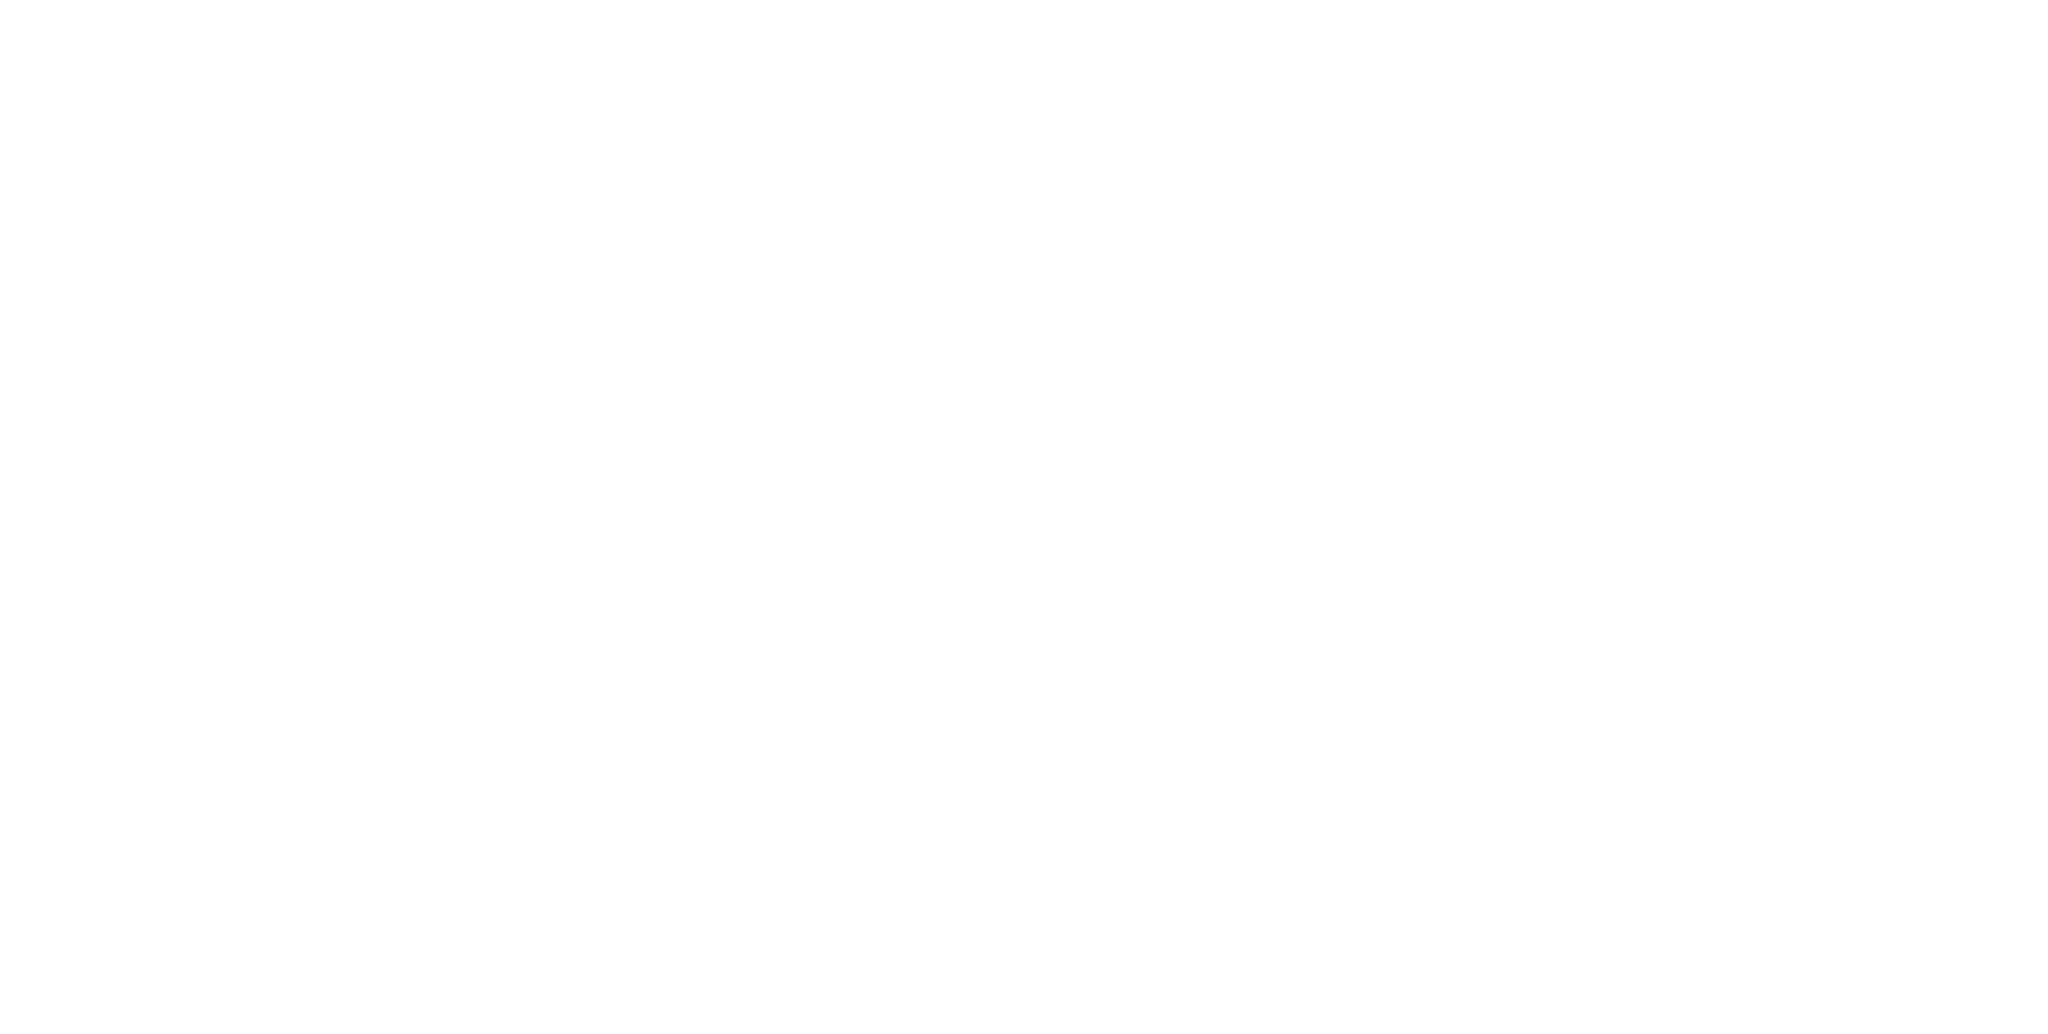
\includegraphics[width=12cm]{diagrams/04/scoped_identifier.svg}

\paragraph{Package}
%TODO

\paragraph{Classi, Interfacce, Enum e Annotazioni}
%TODO

\paragraph{Metodi}
%TODO

\paragraph{Variabili}
%TODO

\paragraph{Dichiarazioni di Tipo}
%TODO

\paragraph{Ereditarieta'}
%TODO

\paragraph{Accesso ai Campi}
%TODO

\paragraph{Chiamata di Metodi}
%TODO

\paragraph{Inclusione}
%TODO

\paragraph{Modificatori}
%TODO
